\documentclass[a4paper,11pt]{scrreprt}
% \usepackage{ngerman}
\usepackage[ngerman]{babel}
\usepackage[utf8x]{inputenc}
\usepackage[T1]{fontenc}
\usepackage{multicol}
\usepackage{ifpdf}
\usepackage[pdftex]{color}
\usepackage{scrhack}
\usepackage{listings}
\usepackage[colorlinks=true,linkcolor=black]{hyperref}
\usepackage{geometry}
\geometry{a4paper,left=30mm,right=20mm, top=26mm, bottom=35mm}

\ifpdf
  \usepackage[pdftex]{graphicx}
\else
  \usepackage[dvips]{graphicx}\fi

\newcommand{\kur}{\textit}
\newcommand{\ul}{\underline}
\newcommand{\bo}{\textbf}

\setcounter{tocdepth}{3}

\newcommand{\format}{\textbf}

\begin{document}

\begin{titlepage}

\vspace*{\fill}
  \begin{center}

\huge \bfseries AUTOSAR \\[2.5cm]

\textsc{\Large SoSe 2015}\\[0.5cm]

\large \today

\vfill

  \end{center}
\end{titlepage}

\begin{itemize}
\item[] \textbf{\large Beitragende:}\\
Daniel Tatzel (DT)\\
Florian Laufenböck (FL)\\
Markus Wildgruber (MW)\\
Philipp Eidenschink (PE)\\
Tim Schmiedl (TimS)\\
Tobias Schwindl (TobiS)
\end{itemize}

\bigskip

\begin{table}[!h]
 	\centering
	\begin{tabular}{|c|c|c|c|}
	\hline
	\textbf{VersionsNr} &  \textbf{Datum} & \textbf{Auslöser} & \textbf{Beschreibung} \\
	\hline
	1.0 & 21.04.2015 & DT & Erster Entwurf \\
	\hline
	\end{tabular}

% \caption{Überarbeitungshistorie}
\end{table}



\chapter{Projekt Beschreibung}

\section{Vernetzte Ballschussanlage}

\begin{itemize}
 \item 1-2 Bricks
 \item Displays Ausgabe
 \item Stop-Taster
 \item Variable Aufteilung unter den Bricks: Stopp-Taste, Auslösung Taste(auch über Ultraschall), Ausgabe
\end{itemize}

\section{Benötigte VFB-Komponenten und Schnittstellen (DT)}

\begin{itemize}
 \item Komponenten
 \begin{itemize}
  \item Application Software Component
  \item Sensor-Actuator Software Component
  \item ECU Abstraction Software Component
 \end{itemize}

 \item Schnittstellen
 \begin{itemize}
  \item Client/Server
  \item Events
  \item Sender/Receiver (auch mit synchronisierung)
 \end{itemize}

\end{itemize}


\section{Namenskonventionen und Standardrückgabtyp (Alle)}

\begin{tabular}{ll}
 Für RTE-Funktionen: & RTE\_<Funktionsname>\_<Portname>\_<Direction> \\
 Für den Rest: & <Komponente>\_<Funktionsname> \\
 \\
 Standardrückgabtyp: & uint32\_t \\
\end{tabular}

\begin{figure}[htbp]
 \centering
 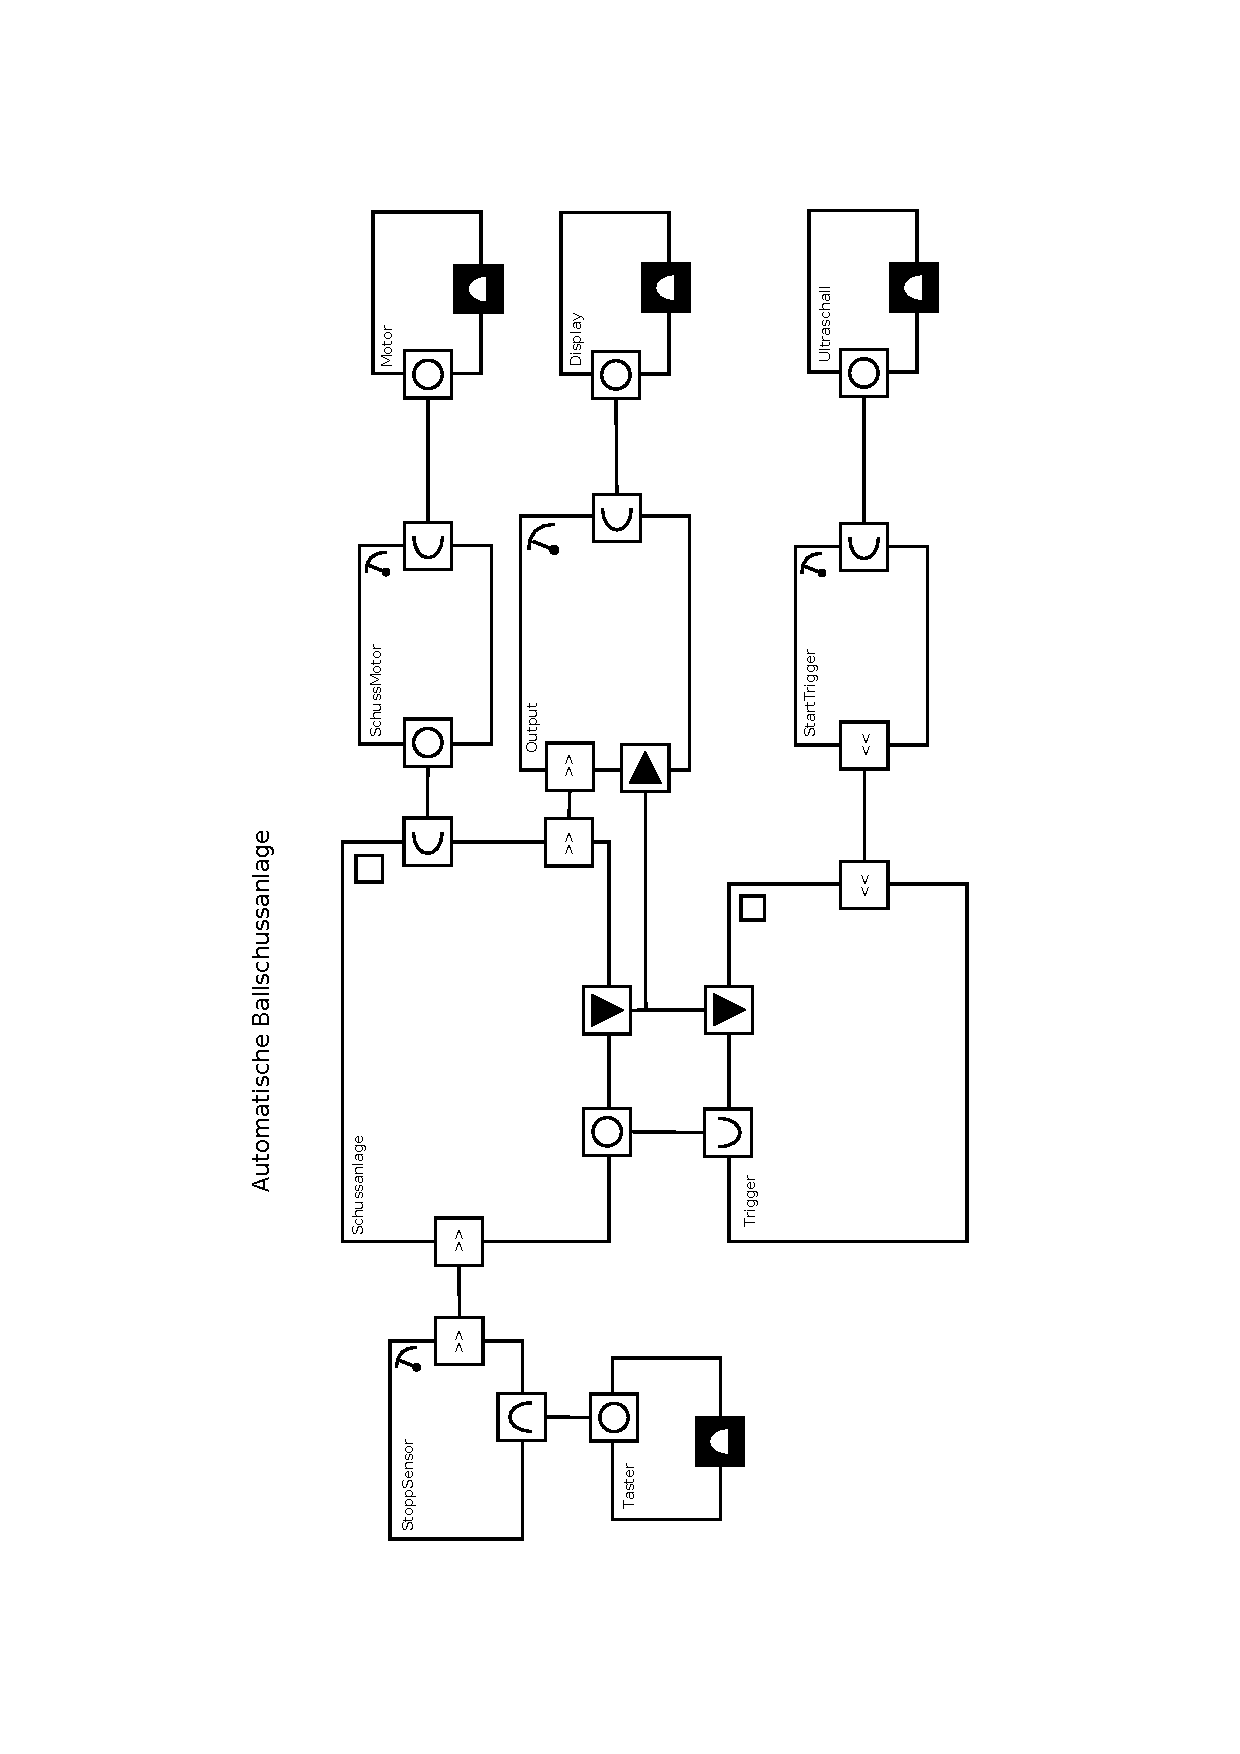
\includegraphics[scale=.75]{./KomponentenDiagramm.pdf}
 \label{fig:komponentendiag}
 \caption{Komponentendiagramm der Ballschussanlage (DT)}
\end{figure}

\chapter{Komponenten-Beschreibung}

\subsection*{Schussanlage (FL)}

\begin{itemize}
 \item Besteht aus einem Task mit zwei Runnables
 \item Erste Runnable für die Abbruch-Bedingung
 \item Zweite Runnable wird durch Trigger gestartet (Schussfreigabe)
 \item Sendet sowohl Event als auch Nachricht an die Output-Einheit
 \item Hohe Priorität
 \item Kein Autostart, kann über den Trigger gestartet werden
\end{itemize}

Benötigt: Task und Event

\subsection*{Trigger (PE)}

\begin{itemize}
 \item Ein Task
 \item Wird zu beginn gestartet (Autostart)
 \item Wartet auf Event vom Ultraschall
 \item Besitzt hohe Priorität
\end{itemize}

Benötigt: Task und Event

\subsection*{Output (MW)}

\begin{itemize}
 \item Task mit niedriger Priorität
 \item Autostart
 \item Wird durch Event von Schussanlage getriggert
 \item Prüft nach Event die empfangene Nachricht
 \item Zeigt Nachricht in Abhängigkeit der empfangen Nachricht an
\end{itemize}

Benötigt: Task und Event

\subsection*{Display (MW)}

Steuert Display an.


\subsection*{SchussMotor (TimS)}

\begin{itemize}
 \item Kein Autostart
 \item Sehr hohe Priorität
 \item Servertask wird durch Schussanlage (client) gestartet
 \item Steuert Motor zum schießen an
\end{itemize}

\subsection*{Motor (TimS)}

Steuert Motor an.

\subsection*{StopSensor (TobiS)}

\begin{itemize}
 \item Autostart
 \item Sehr hohe Priorität
 \item Prüft Taster
 \item Setzt Event für Schussanlage
\end{itemize}

Benötigt: Task, Timer und Event

\subsection*{Taster (TobiS)}

Prüft Taster Wert.

\subsection*{StartTrigger (TobiS)}

\begin{itemize}
 \item Task zum Erkennen von Zielen
 \item Autostart
 \item Sehr hohe Priorität
 \item Sendet Event an Trigger
 \item Erkennung durch periodische Abfrage
\end{itemize}

Benötigt: Task und Timer

\subsection*{Ultraschall (TobiS)}

Prüft Ultraschall Wert.

\end{document}
